\section{Business Process Modeling Notation (BPMN)}

\subsection{¿Qué es?}

Al interior de una organización es importante documentar y especificar los diferentes procesos que se deben llevar a cabo. A menudo, se suelen utilizar diagramas de flujo o incluso descripciones textuales. Desafortunadamente, estas técnicas se quedan cortas a la hora de describir procesos mas complejos, y mas aún cuando cada organización define su propia notación, dificultando el entendimiento de los diferentes modelos que se realizan al interior de la organización. Es por esto que se hace necesario crear una notación estándar y especifica para describir este tipo de procesos.

BPMN, Business Process Modeling Notation, es precisamente el estándar que se viene adoptando a nivel masivo para la creación y descripción de los diferentes procesos que hacen parte del funcionamiento de las diferentes organizaciones.


Con el estándar BPMN, se tienen en cuenta diferentes elementos básicos que sirven como herramientas para crear y estructurar los diferentes modelos que se quieran hacer. Estos elementos solo describen una forma básica de uso, pues BPMN permite personalizar los elementos a utilizar, siempre y cuando los cambios realizados no dificulten el proceso de entendimiento de los modelos.

\subsection{Enlaces}

Los enlaces sirven para unir o bifurcar el flujo de secuencia de un modelo. Son utilizadas cuando es necesario tomar algún tipo de decisión que lleve a tomar uno o varios caminos alternos. Existen varios tipos de enlaces, como lo son los enlaces exclusivos, paralelos, inclusivos y complejos.

\subsubsection{Enlaces exclusivos}

Los enlaces exclusivos se utilizan cuando es necesario tomar una decisión para tomar un único camino. Se modela mediante un diamante vacío o un diamante con una ``X'' en su interior. La figura \ref{fig:gateway_exclusivo} muestra un ejemplo de uso de este enlace.

\begin{figure}[!htb]
  \begin{center}
    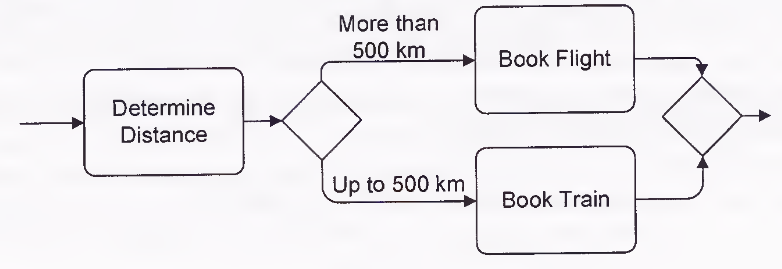
\includegraphics[width=11cm]{./imagenes/gateway_exclusivo.png}
    \caption{Ejemplo de uso del enlace exclusivo}
    \label{fig:gateway_exclusivo}
  \end{center}
\end{figure}

En este caso, se realiza la actividad \textit{Determinar distancia} y se decide que tipo de medio de transporte se debe utilizar. Nótese que luego de realizar la reserva, se vuelve a unir el flujo de secuencia del modelo, ya que no se sabe en la práctica cual de las 2 alternativas será la seleccionada.

\subsubsection{Enlaces paralelos}

El enlace paralelo se utiliza cuando es necesario realizar varias actividades en paralelo, partiendo el flujo de secuencia en varios flujos que luego deben reunirse. Se modela mediante un diamante con un signo más (+) en su interior.

\begin{figure}[!htb]
  \begin{center}
    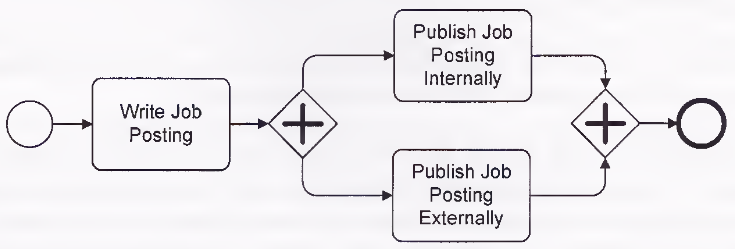
\includegraphics[width=11cm]{./imagenes/gateway_paralelo.png}
    \caption{Ejemplo de uso del enlace paralelo}
    \label{fig:gateway_paralelo}
  \end{center}
\end{figure}

En la figura \ref{fig:gateway_paralelo} se ve un ejemplo de uso de este enlace. Aquí, luego de que se redacta la oferta de trabajo, le procede a publicarla, tanto interna como externamente. En este caso, se utiliza el enlace paralelo para agilizar el proceso de publicación.

\subsubsection{Enlaces inclusivos}

Este enlace se utiliza cuando es posible tomar una o varias decisiones en el flujo de procesos. Se modela mediante un diamante con una letra ``O'' en su interior.

\begin{figure}[!htb]
  \begin{center}
    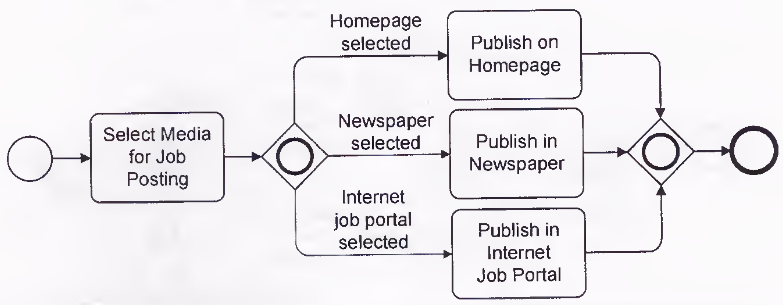
\includegraphics[width=11cm]{./imagenes/gateway_inclusivo.png}
    \caption{Ejemplo de uso del enlace inclusivo}
    \label{fig:gateway_inclusivo}
  \end{center}
\end{figure}

En la figura \ref{fig:gateway_inclusivo} se ve un ejemplo de uso en donde a partir de la actividad ``Seleccionar medio para publicar oferta de trabajo'' se pueden seleccionar una o varias opciones. Cualquier combinación de opciones, que al menos contenga una opción, es válida.

\subsubsection{Enlaces complejos}

Estos enlaces, que no son tan comunes, son utilizados cuando existen reglas mas especificas para unir o separar el flujo de proceso. Se modela mediante un diamante con una estrella (*) en su interior, acompañado de una nota que refleja la regla a seguir.

\begin{figure}[!htb]
  \begin{center}
    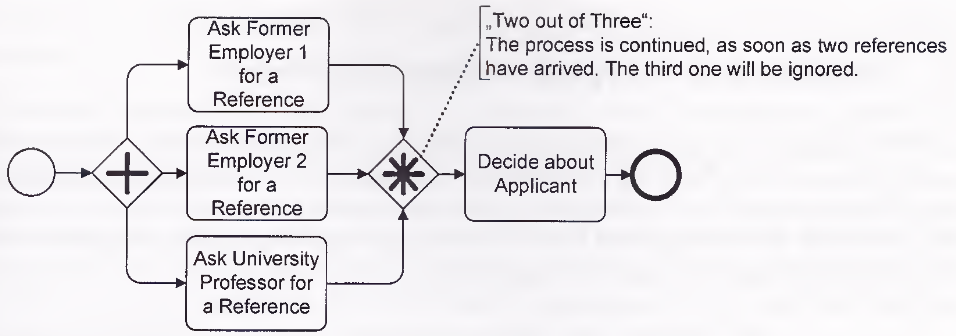
\includegraphics[width=11cm]{./imagenes/gateway_complejo.png}
    \caption{Ejemplo de uso del enlace complejo}
    \label{fig:gateway_complejo}
  \end{center}
\end{figure}

En el ejemplo mostrado en la figura \ref{fig:gateway_complejo}, se requiere la referencia de 2 empleadores previos y de la universidad. En realidad, solo son necesarias dos referencias, pero para estar seguros se piden tres, por lo que tan pronto como llegan las primeras 2 referencias, la tercera puede ser ignorada sin mayor problema.

\subsection{Colaboración}

A menudo, en un proceso intervienen diferentes partes interesadas (\textbf{\textit{Stakeholders}}) y es necesario ver el proceso de manera global, de manera que el paso de mensajes entre las partes implicadas sea mas claro. A este tipo de diagramas se les llama \textbf{diagrama de colaboración}

La figura \ref{fig:diagrama_colaboracion} muestra como es la interacción entre un aspirante y una empresa en el proceso de acceder a una oferta de empleo. Puede verse como, entre las actividades que ejecuta cada una de las partes, existe un paso de mensaje que une ambos procesos. Esta unión se representa por una flecha con linea punteada, donde un extremo tiene un circulo y el otro una flecha vacia que indica la dirección del mensaje.

\begin{figure}[!htb]
  \begin{center}
    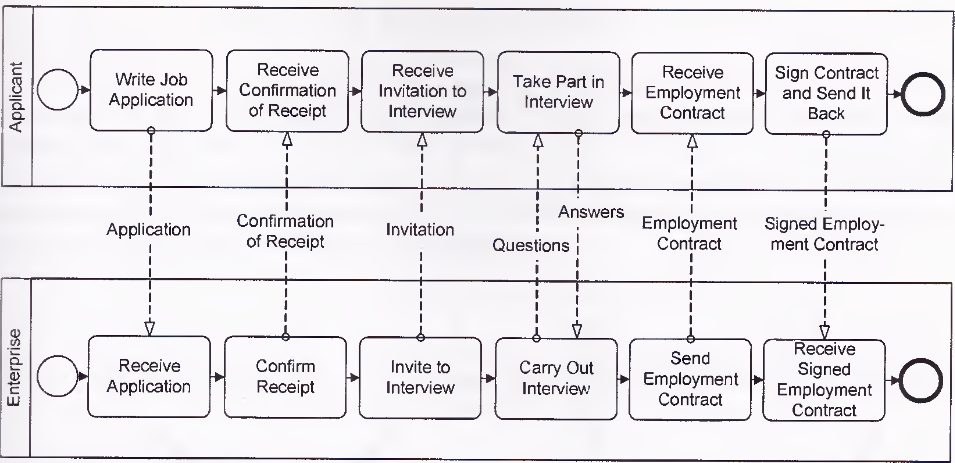
\includegraphics[width=11cm]{./imagenes/diagrama_colaboracion.png}
    \caption{Ejemplo de diagrama de colaboración}
    \label{fig:diagrama_colaboracion}
  \end{center}
\end{figure}

Por ejemplo, la actividad ``Recibir solicitud'' recibe un mensaje de la actividad ``Redactar solicitud de empleo'', por lo cual esta actividad (recibir solicitud) no puede iniciar si el aspirante no envía su solicitud. Esto significa que los mensajes deben ser respetados y una actividad no puede realizarse si le falta algún mensaje de entrada.

Sin embargo, en estos casos solo se conoce el proceso que sigue la empresa, por lo que es común representar a las partes externas como una caja negra (figura \ref{fig:diagrama_colaboracion_caja_negra}).

\begin{figure}[!htb]
  \begin{center}
    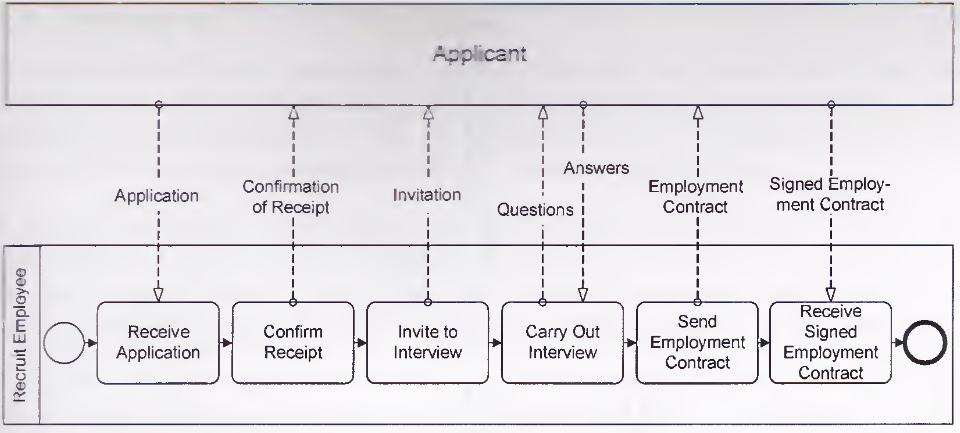
\includegraphics[width=11cm]{./imagenes/diagrama_colaboracion_caja_negra.png}
    \caption{Ejemplo de diagrama de colaboración con caja negra}
    \label{fig:diagrama_colaboracion_caja_negra}
  \end{center}
\end{figure}

\subsection{Eventos}

\subsection{Actividades}

\subsection{Excepciones}

\subsection{Transacciones}

\subsection{Objetos de datos}

\subsection{Coreografía}

\subsection{Conversacion}
